\documentclass[letter,12pt]{article}
%\usepackage[letterpaper,right=1in,left=1in,top=1in,bottom=1in]{geometry}
\usepackage[letterpaper,right=1.25in,left=1.25in,top=1.25in,bottom=1.25in]{geometry}
\usepackage[longnamesfirst, sort]{natbib}\bibpunct{(}{)}{,}{a}{}{,}
\usepackage{ae} % or {zefonts}
\usepackage[T1]{fontenc}
\usepackage[ansinew]{inputenc}
\usepackage{amsmath}
\usepackage{amssymb}
\usepackage{url}
\usepackage{lscape} %landcape pages support
\usepackage{setspace} %allows to change linespacing
%\setstretch{2} %linespacing
%\onehalfspacing
%\doublespacing

% avoid clubs and widows
\clubpenalty=9000 \widowpenalty=9000
% \displaywidowpenalty=9999

\usepackage[pdftex]{graphicx}
%\usepackage{graphicx}
\graphicspath{"c:/data"}
\usepackage{color}
%\usepackage[colorlinks]{hyperref}
\usepackage{tikz} % Easier syntax to draw pgf files (invokes pgf automatically)
\usetikzlibrary{arrows,shapes.geometric}
\usepackage{pgfmath}

\usepackage{multirow} %allows multiple rows in tables
\usepackage{rotating}% allows sideways tables or other stuff

%for submission: sends figs and tables to last pages, other turns footnotes to endnotes
%if endnotes used, place \listofendnotes where you want the endnotes to appear (it must be after the last endnote).
%el archivo "endfloat.cfg" (disponible en C:...\miktex\tex\latex\endfloat) debe guardarse en el directorio de trabajo para jalar sidewaystable al final con dem�s tablas
%%\RequirePackage[nomarkers,nolists]{endfloat}
%%\RequirePackage{endnotes}
%%\let\footnote=\endnote
%%\newcommand{\listofendnotes}{
%%   \begingroup
%%   \parindent 0pt
%%   \parskip 2ex
%%   \def\enotesize{\normalsize}
%%   \theendnotes
%%   \endgroup
%%}

% titlepage without author and date
%\renewcommand{\maketitle}{
%%   \begin{spacing}{1.5}
%%   \centering
%%   \LARGE{\textbf{\@title}}
%%   \end{spacing}
%%}

% to change margins in a section -- type \begin{changemargin}{deltaLEFT}{deltaRIGHT}
\def\changemargin#1#2{\list{}{\rightmargin#2\leftmargin#1}\item[]}
\let\endchangemargin=\endlist

%permiten a�adir espacio arriba o abajo del texto de un rengl�n en una tabla
\newcommand\T{\rule{0pt}{2.6ex}}         % Top strut at least 2.6ex
\newcommand\B{\rule[�1.2ex]{0pt}{0pt}}   % Bottom strut at least 2.6ex
%usage
%\begin{tabular}[t]{|c|c|}
% \hline
% \multicolumn{2}{|c|}{Laplace transforms\T\B}  \\\hline
% $f(t)$ \T        & $(p)$ \B                     \\\hline
% $\delta(t)$      & $1$ \T                       \\[.5ex]
% $\cos\omega_0t$  & $\frac{p}{p^2+\omega_0^2\B}$ \\\hline
%\end{tabular}

%\bibdata{c://mydocs//1new//}

%adds comma-separator to thousands
%\usepackage[np]{numprint}

\usepackage{tikz} % Easier syntax to draw pgf files (invokes pgf automatically)
\usetikzlibrary{arrows}

\begin{document}

\title{Voting and sincerity. Ideal point drift and strategy in a regulatory board\thanks{
     Paper presented at the Annual Meeting of the American Political Science Association,
     Toronto, Canada, September 5, 2009. We are grateful to Omar Alejandre for sharing his
     data on originating IFE committees. Authors are responsible for any errors.} }
\author{Eric Magar\\ITAM\\ {\small \url{emagar@itam.mx}}
    \and Guillermo Rosas\\Washington Univ., St.\ Louis\\ {\small \url{grosas@wustl.edu}}
    \and Federico Est�vez\\ITAM\\ {\small\url{festevez@itam.mx}}}
\date{\today}
\maketitle
% \thispagestyle{empty}  %% removes page numbers
% \pagestyle{empty}      %% removes page numbers part 2

%\begin{center}\textbf{Draft} --- not for circulation --- comments very welcome\end{center}

\begin{abstract}
\noindent We use a dynamic item response theory model
\citep{martin.quinn.2002} to investigate ideal point stability in
Mexico's IFE, an election regulatory board. Results indicate that
stability is not predominant, that most board members moved
considerably a good deal of the time. We discuss how theories of
representation view movement and show that some of the drift we
detected is in fact associated with systematic factors. Evidence
suggests that movement and strategic considerations associated with
representation correlate, contradicting the standard assumption
of sincere voting.
\end{abstract}

%FRAMING FUTURO
% Clinton Jackman Rivers dicen que sin sincere voting Nominate est� mal (creo).
% En realidad no est� mal el n�mero, pero s� su interpretaci�n.
% Sin voto sincero Nominate (y Theta) deja de ser medida de ideolog�a
% para volverse un mero resumen de los determinantes del voto.
% Para entenderlo hay que entender los determinantes.

The life tenure of Supreme Court Justices that is key to judicial
independence \citep{hamilton.1788} also makes the Court a singular
voting body. Unlike members of assemblies whose careers depend upon
securing and renewing the sympathy of others, Justices are free to
follow their sincere preferences when ruling, regardless of whether
others like the ruling or not. Recent developments in the field of
ideal point estimation
\citep{clinton.jackman.rivers.2004,martin.quinn.2002} have provided
a method to measure temporal shifts in the voting records of Supreme
Court members. Estimates reveal that, in fact, many Justices have
changed voting criteria, often substantially, relative to other
members over the course of their careers.

Members of other assemblies not formally insulated from external
political pressure are not as lucky. Members of Congress
\citep{mayhew.1974}, of congressional committees
\citep{weingast.marshall.1988}, of regulatory boards
\citep{mcnollgast.1987}, of lower courts \citep{gely.spiller.1990},
all are primarily moved by those they represent. Scholarship has
showed that if personal beliefs matter at all in how members of
representative bodies vote, they are relegated by much more
important and systematic forces. Representatives' votes are driven
by the will and preferences of constituents, mediated by relevant
institutions. If follows that if neither the will of constituents
nor mediating circumstances change, representatives' voting record
should remain unchanged, reflecting an equilibrium of forces
supporting it.

We seek evidence of stability in representative bodies by using
Martin and Quinn's \citeyearpar{martin.quinn.2002} dynamic
estimation method for ideal points in a regulatory board. The case
study is Mexico's Federal Election Institute (IFE), whose Council
General decides all aspects of election regulation and oversaw
Mexico's transition to a system of competitive elections. We argued
in our previous work \citep{estevez.magar.rosas.2008} that IFE is an
agent of the congressional parties who appoint and can impeach the
council's nine members. To our surprise, members' voting records
shift as much as those in the U.S.\ Supreme Court, a finding we
discuss in section 1 of the paper. Movement in many cases consists
of continuous monotonic drift in ideal points over time, not simple
shocks followed by a return to a central tendency.

We have been careful to write `voting record' and not `preference'
or even `ideology' because, as we discuss in section 2, ideal points
recovered by scaling techniques are valid measures of personal
beliefs in quite stringent conditions only. Otherwise it is more
prudent to take them for what they are, a statistic of a member's
voting record. Even if not read as ideology, this record remains
useful for many reasons. Section 3 offers a discussion of strategic
factors that should be behind ideal point movement in representative
bodies. These factors are associated with constituent
representation, with the structure and process of decision-making,
and with vote trading. Factor identification sets the stage to
formulate a model accounting for ideal point drift that can also be
estimated in our future research. Section 4 analyzes movement
patterns finding evidence that they are associated with these
factors, some at least. Section 5 concludes.

\section{Dynamic ideal point estimation}\label{S:model}

Scaling techniques to infer ideal points rely on a standard spatial
model of voting \citep{black.1958,poole.rosenthal.1997}. The
approach assumes that policy and preferences can be mapped in the
same space
--- as points in a line or plane --- while distance determines
utility and voting. Voters in this context differ from one another
in their locations in the policy space, each choosing the
alternative closer to his or her ideal point. The aim is to use
observed votes to estimate voters' ideal points and other parameters
of interest.

We specified a one-dimensional version of the model. In accordance
with the spatial approach, voting `aye' ($y=1$) or
`nay' ($y=0$) on an issue %(we here drop $i$ subscripts for convenience)
depends on the relative locations of policy outcomes vis-�-vis voter
$j$'s ideal point $x_j$ in space. Voting is sincere---we revisit
this assumption in section \ref{S:explaining}. If $x^{(A)},x^{(N)}
\in \mathbb{R}$ denote the outcomes of the aye and the nay votes,
respectively, it is their midpoint $m=(x^{(A)}+x^{(N)})/2$ that
matters for analysis. The voter will prefer the alternative falling
on the same side of $m$ as his or her ideal point. Formally, $j$'s
vote propensity is $y^*_{j}= \delta(x_j - m)
+\text{error}$,\footnote{Item response theory models designed to
infer a latent trait (eg. intellectual ability or ideology) from
allegedly related subjects' traits (eg. answers to items in the GRE
test or roll call votes) are routinely used in ideal point
estimation. In IRT context, $m$ is the item difficulty parameter and
$x_j$ the ability parameter. When relying on quadratic utility
functions, as we do, $\delta = -2(x^{(A)} - x^{(N)})$. Estimation
does not recover the coordinates of the aye and nay policy
alternatives, only their midpoint. As the distance between them
increases, their choice becomes likelier to arouse passions between
judges, which is precisely what $\delta$ is intended to capture.}
where $x_j-m$ is the deterministic part of voting, $\text{error}$ is
random noise, and $\delta \in \mathbb{R}$ is a discriminator. The
$\delta$'s sign fixes issue polarity (so that conservatives can also
vote nay) while its size in absolute value weighs the importance of
the systematic part of the vote relative to the random part. In the
extreme $\delta=0$ voting is entirely determined by the random
disturbance. The voting rule is $y_{j}=1 \iff y^*_{j} \geq 0$,
otherwise $y_{j}=0$.

We analyze all contested roll call votes held at IFE's Council
General between October 1996 and December 2007. A vote qualifies as
divided when, ignoring abstentions and absences, at least one
councilor voted contrary to the rest. This filter removed 1,641
unanimous votes failing to distinguish councilors from one another
from the dataset, leaving our empirical base with 770 roll call
votes, 35 percent of all.

\begin{figure}
 \begin{center}
    \includegraphics[width=11cm]{c:/data/graphs/all+divVotsSemestre.pdf} \\
 \caption{\emph{Universe of roll-call votes and analyzed subset.}
 Left dotted line marks a partial Council renewal, the right one a
 full renewal. Stars on x-axis mark federal election semesters.}\label{F:all+div}
 \end{center}
\end{figure}

The Council General, a nine-member board, was newly appointed at the
start of the period we scrutinize, and suffered a partial renewal in
December 2000, when two members quit early to assume executive
appointments, and a mandatory full replacement in October 2003;
replacements appear as vertical dotted lines in Figure
\ref{F:all+div} distinguishing three periods. Period III ends with
the resignation of then Councilor president Ugalde in the aftermath
of the 2006 presidential election contestation. Semester variations
in non-unanimous tendencies in the Council are patent, ranging from
a minimum of 7 percent divided votes (in the second semester 2007,
also having an outlying number of total votes) to a maximum of 68
percent (in the first of 2003).

We specified a version of Martin and Quinn's
\citeyearpar{martin.quinn.2002} dynamic IRT model to estimate
members' semestral ideal points from contested roll calls. At the
core of their model is the assumption that a member's ideal point
may not be constant in the course of a study, as standard IRT models
assume. Estimating the model separately for different discrete time
periods (semesters in our case) would be an obvious alternative, but
one assuming that a member's ideal point at time $t$ is independent
from her ideal point at time $t-1$. Instead, the dynamic model
posits a temporal dependency for member $j$'s ideal point $x$ in
semester $t$, such that $x_{j,t} \sim \mathrm{N}( x_{j,t-1},S )$
where $S$, the slack, governs how much past determines present:
$S=0$ makes the model equivalent to the classic (static), while $S
\to \infty$ assumes time independence. We ran the model with
different slack values, opting for $S=.02$ in the results we
present, the standard deviation of which is one-fourteenth of the
full left-right spectrum we define below. We detect drift in ideal
points even with this small slack values.\footnote{Using larger
values for $S$ did not change the direction nor magnitude of changes
in the full periods covered, but allowed for high one-semester
volatility. Our choice of $S=.02$ smoothes the short-term trends.}

A separate model was estimated for period III because it shares no
members with earlier periods; periods I and II, sharing 7 out of 11
members, were estimated jointly. Small committees raise
complications for model estimation \citep{londregan.2000b}. With
$J=9$ councilors and $I=148$ items (all votes in period III), $J
\times I =1332$ data points are used to estimate $2 \times I+ J =
305$ parameters. With only slightly more than 4 observations per
parameter, likelihood-based estimation becomes problematic for a
case such as IFE. Bayesian methods, implemented via MCMC simulation
\citep{clinton.jackman.rivers.2004}, can overcome such
problems.\footnote{Three chains were updated 200 thousand times
each, preserving every 100th observation from the second half. We
thus obtained a sample of $3\times1000=3000$ posterior simulations
to derive our results. Gelman and Hill's
\citeyearpar{gelman.hill.2007} $\hat{R} \approx 1$, suggesting that
the chains had converged towards a steady state. WinBUGS
\citep{winbugs.2000} was used for model estimation, invoking it from
R \citep{r.cite.2006}, also used for post-analysis. The appendix to
the paper provides a sample of our code.}

The Bayesian approach requires prior probabilities for un-modeled
parameters to be estimated: $x_{j,0}$ (the start, of ideal point
series at $t=0$), $m_i$ and $\delta_i$ ($i=1\cdots I$ and $j=1\cdots
J$). We adopted non-informative priors --- ie. a zero-mean normal
distribution with variance one --- for all parameters except two
councilors' starting ideal points. These --- inferring from
\citet{estevez.magar.rosas.2008}\footnote{In periods I and II,
C�rdenas anchors one end with $x_j \sim N(-2,.25)$ while Barrag�n
the other with $x_j \sim N(2,.25)$; in period III Gonz�lez Luna and
G�mez Alc�ntar assume the extremes. We avoid speaking of `left' and
`right' because the policy scale is IFE-specific and these are
misleading terms.} --- were instead given semi-informative priors to
give the arbitrary scale on which estimates are mapped a unit and a
sense of what `North' and `South' actually mean.

\section{Drift in a regulatory council}\label{S:results}

Figure \ref{F:allwMedian} reports the central tendency of the
posterior $x_{j,t}$ density, our dynamic estimate of ideal points.
(For member-by-member results, including a measure of uncertainty,
see Appendix 2.) Color identifies members' sponsoring parties, a key
variable driving voting at IFE \citep{estevez.magar.rosas.2008}. A
good degree of drift in ideal points is always evident at IFE,
although periods are different in important ways.

\begin{figure}
 \begin{center}
  \begin{tabular}{cc}
    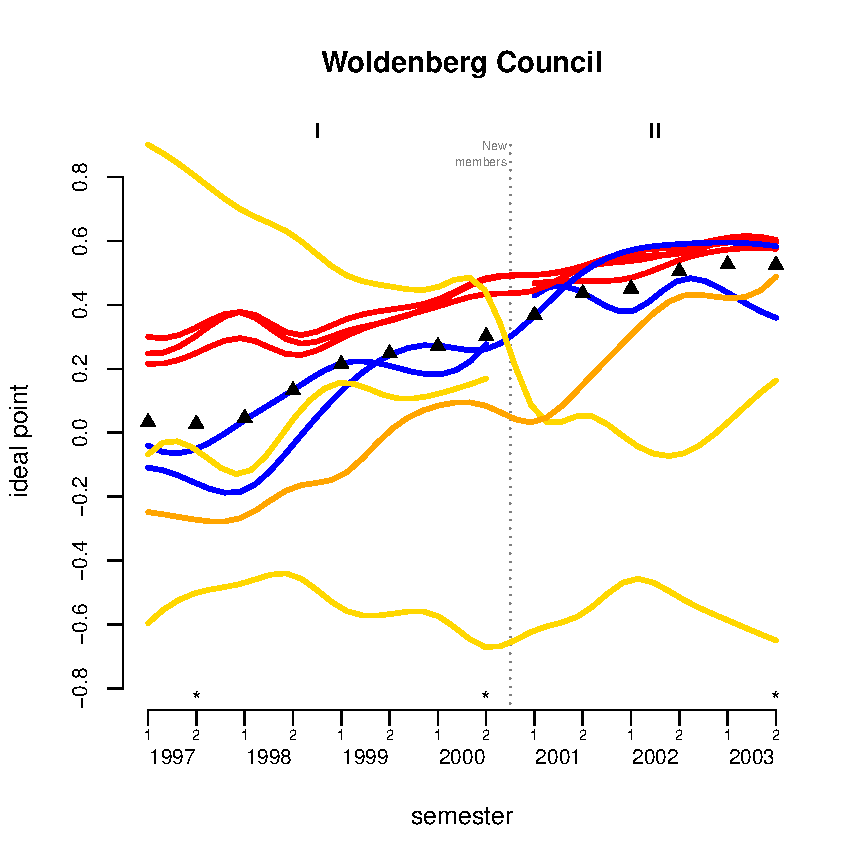
\includegraphics[width=.48\textwidth]{c:/data/graphs/allWdynNoNames.pdf} &
    \includegraphics[width=.48\textwidth]{c:/data/graphs/allUdynNoNames.pdf} \\
  \end{tabular}
  \caption{\emph{Councilors' ideal points in two Councils.} Lines
  report the median of the councilor's posterior density, colors indicating
  councilor's sponsoring party: blue = PAN, red = PRI, gold = PRD,
  green = Green. Triangles report expected Council median. Stars in
  x-axis mark federal election semesters.}\label{F:allwMedian}
 \end{center}
\end{figure}

Only two members can be said to have something like flat lines in
periods I and II --- the southernmost yellow and the blue present in
II only. Changes in one semester were followed by readjustment in
the next few, so they ended more or less where each had started.
This is presumably the pattern expected for ideal point stability,
short deviations caused by idiosyncratic or in any case short-term
shocks. All other members experienced, in different degrees,
monotonic change in the location of ideal points throughout all or
nearly all their tenure. This is less acute among red members: after
a slight readjustment in course in the first semester 1998, they
began drifting slowly, but constantly northward. Both councilors who
quit early had slightly steeper drift trajectories, also in north
direction. But it was the remainder three councilors who experienced
the most pronounced change in ideal points: the only member with a
southward path went from the extreme to about the center of the
spectrum, the most spectacular change; the other two (blue and
yellow) abandoned south-of-center positions nearly monotonically to
distinctly join the red crowd in in the second half of their tenure.

While drift or monotonic change in ideal points was also present in
period III, it was more exceptional than before. The green councilor
drifted constantly until it reversed gears in the last two
semesters. It is important to note that the last semester in period
III was frankly anomalous because congressional parties were openly
negotiating the premature removal of several Councilors after the
2006 post-election dispute. So movement in the last semester of the
series, if not the last year, is subject to unusual noise,
discernible in the erratic moves by many members. Dropping the last
year leaves the green member unadjusted after a distinct drift. The
same is true for the second red from top to bottom, and less so for
the bottom red when the full period III is considered. The rest had
mild drift and/or experienced readjustments.

\begin{figure}
 \begin{center}
  \begin{tabular}{cc}
    \includegraphics[width=.48\textwidth]{c:/data/graphs/driftW.pdf} &
    \includegraphics[width=.48\textwidth]{c:/data/graphs/driftU.pdf} \\
  \end{tabular}
 \caption{\emph{Ideal point drift patterns.} Grey bands indicate, to each side of
 white 45� line, mean absolute drift in period plus one standard deviation; black points fall
 beyond. Green circles start drift trajectory for one councilor, red ones end it.}\label{F:drift}
 \end{center}
\end{figure}

Figure \ref{F:drift} conveys different perspective on drift,
plotting members' $x_{j,t}$ against $x_{j,t+1}$. Any semester
movement will pull the point away from the white, and light dark
lines connect points for the same member to give a picture of
individual movement patterns. The width of the grey band covers the
mean absolute change in the period covered by the chart plus one
standard deviation, black colored points falling beyond. Green and
red contours indicate the start and end of a member's trajectory,
information we elaborate on below. Charts show differences between
the councils. Note that in periods I and II two, three, or even
black points are connected, indicating repeated abnormal drift by
the same people, all but one above the 45� line (the northward
general trend seen in figure \ref{F:allwMedian}). Note also that
bigger inter-semester moves in period III widen the grey bar, and
that some black points are connected, but these tend to be on both
sides of the grey bar --- abnormal returns after abnormal shifts.
Movement in periods I and II appears more indicative of ideal point
drift. The next section elaborates some possible explanations of
such movement in a representative voting body.

\section{Explaining ideal point drift}\label{S:explaining}

What is behind ideal point movement and what does it mean? We now
turn to the literature on voting in committees large and small in
searh for answers. Ideal points reflect members' ``operational
preferences'' \citep{cox.2001}, in turn theorized as a mix of four
general factors: personal belief; constituents' pressure; side
payments; and structure and process.

\subsection{Personal belief}

Poole and Rosenthal \citeyearpar{poole.rosenthal.1997} explicitly
interpret the scores recovered by their WNominate algorithm as
estimates of members' ideology. Their work was received with such
enthusiasm that the interpretation of scores as cardinal
translations of the `liberal-conservative' divide is accepted by
many with little discussion. But the interpretation remains
questionable. The translation of legislative scaling scores into
degrees of ideology will be valid when personal belief is the sole
determinant of voting. And this occurs if, and only if, the other
three vote-influencing factors are absent or their effect
negligible: when constituents are unwilling or unable to exert
pressure; and vote buying is precluded or unfeasible; and committee
institutions are neutral. The fulfilment of this triad boils down to
the condition of \emph{sincere voting} --- a standard assumption of
voting models that remains quite stringent a condition.

Another way of looking at the problem at hand is by posing that
strategic behavior invalidates sincere voting. Positive political
theory has shown the near ubiquity and the many guises of strategy
in politics, how strategic actors very often fail to choose the
best-liked alternatives if that will produce a better outcome down
the game tree. All determinants of voting in committees except
personal belief are incarnations of strategic behavior.

\subsection{Representation and constituents' pressure}

The first incarnation is grounded in relations of representation and
delegation in politics and other domains. Legislators constantly
delegate policy-making power to experts
\citep{kiewiet.mccubbins.1991}. The primary advantage of this type
of delegation is that legislators may rely on agents to formulate
policies they themselves would have if they had the time to do it.
The primary drawback is that agents can act against the interest of
legislators, leaving them worse than if they had not delegated
powers. The classic solution to cut agency costs combines careful
screening of candidates and sanctions to non-compliant agents. In
appointing agents, legislators --- more generally principals or
constituents --- will stack the deck in favor of compliance since
before the contract begins by choosing types with policy
predispositions similar to their own \citep{mcnollgast.1987}. And
principals usually retain the powers to penalize agents acting
against their interests, such as budget cuts or even the removal of
wrongdoers. To the extent that agents value their job, threats to
use this ``big club behind the door'' \citep{weingast.1984} ought to
reduce the gap remaining between agent's and principal's goals.

All this renders tensions between an agent's personal beliefs and
principal's interests minimal or at least workable: if screening
fails to sufficiently align the two \emph{ex-ante}, credible
\emph{ex-post} sanctions ensure the that the latter prevail in the
end. This view is encapsulated in Mayhew's \citeyearpar{mayhew.1974}
seminal model of representatives as automatons concerned only in
keeping constituents pleased. A member's operational preferences in
the Mayhewvian mold will shift only in response to changes in
constituency interests. Redistricting, or sharp changes in the
social-demographic profile of the district, or the organization of a
latent interest group with resources to harm the agent, all are
examples of potential shocks to members' ideal points.

\subsection{Structure and process}

The second incarnation of strategic behavior is grounded in agenda
setting. Early models of voting in assemblies
\citep[eg.][]{mckelvey.1976} consisted of a bare majority rule with
no institutional structure such as leaders, specialized committees
or parties. Cox and McCubbins \citeyearpar{cox.mccubbins.2005} have
argued that democratic legislatures in their infancy conformed well
to that picture, but legislative institutions redistributing agenda
power evolved as responses to several collective dilemmas: ``even
though voting power in democratic legislatures is everywhere equal,
proposal and veto power are everywhere unequal'' (p.\ 9).

With closed agendas giving members a sequence of specific
alternatives to vote on with no chance of proposing amendments,
incentives for sophisticated voting appear inevitably
\citep{satterthwaite.1975}. Sophisticated voting consists of
supporting the alternative you rank second (or some middle
preference) when you expect your favorite will lose. More
specifically, it happens in a sequence of paired votes when, in each
step, voters choose an optimal strategy in light of what others will
do in the game. The classic example \citep{enelow.koehler.1980}
involves a relatively extreme proposal $P$, such as the one IFE
discussed on 16 December 1997 for the Council president to have the
power to name and remove key bureaucratic agents dealing with the
media, international affairs, and internal oversight. Although
creating such units was desirable for the majority, it was also
anticipated that, giving appointing an removal power to the
president only, $P$ would be defeated by the status quo $Q$. In an
attempt to save the issue, an amendment $E$ more attractive to
moderates was offered. The motion established that agents be named
and removed by the Council general from a slate of candidates
proposed by the president. In spatial terms, the left-to-right
ordering of the alternatives was Q--E--P, the right favoring a
stronger presidency, the left Council supremacy.

\begin{figure}
 \begin{center}
     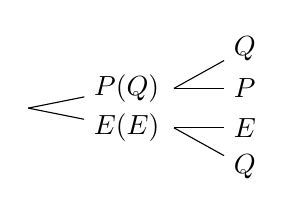
\begin{tikzpicture}
     \node at (2,1.5) (pq) {$P(Q)$};
     \node at (2,1) (ee) {$E(E)$};
     \node at (3.5,2) (qu) {$Q$};
     \node at (3.5,1.5) (p) {$P$};
     \node at (3.5,1) (e) {$E$};
     \node at (3.5,.5) (qd) {$Q$};
     \path[-] (.75,1.25) edge (pq)
              (.75,1.25) edge (ee)
              (pq)+(.6,0) edge (qu)
              (pq)+(.6,0) edge (p)
              (ee)+(.6,0) edge (e)
              (ee)+(.6,0) edge (qd);
     \end{tikzpicture}
  \caption{\emph{A voting agenda and sophisticated voting.} See text.}\label{F:sophisVote}
 \end{center}
\end{figure}

We illustrate with an agenda portrayed in figure \ref{F:sophisVote}
pitting first $P$ against $E$, then the winner against $Q$ (ignore
terms in parentheses for now).\footnote{The agenda that was actually
followed for the referred case was $Q$ against $P$ then, if the
latter won, $P$ against $E$. It also illustrates sophisticated
voting, but does so less eloquently than the example in the text.}
Assuming that the initial result with sincere voting is that $E$
wins, all members to the right of $(E+P)/2$ (the midpoint of $E$
against $P$) would have voted for $P$ first, and would do it for $E$
in the second stage; moderates with ideal points between $(Q+E)/2$
and $(P+E)/2$ would have voted for $E$ first and would do the same
second; and all to the left of $(Q+E)/2$ would have voted for $E$
first then for $Q$. The sincere outcome would be $E$. With this
agenda, however, voting sincerely is not optimal for the left. Since
$E$ beats $Q$ but $Q$ beats $P$ in the possible second stage votes,
the first stage vote should be seen, from the strategic perspective,
not as $P$ against $E$ but as $Q$ against $E$ \citep[parenthesized
in figure \ref{F:sophisVote},][]{schwartz.1987}. Leftists do better
voting for radical proposal $P$ in the first stage because, if the
right votes sincerely, that guarantees the triumph of $Q$. And if
the right also espouses sophisticated behavior, it would opt for $E$
in the first stage to avoid the victory of its worse alternative
later.

The effect on voting from the left, moderates, and right is quite
straightforward: if sincerely they respectively choose $E$, $E$, and
$P$ in the first vote, they sophisticatedly do it for $P$, $E$, and
$E$, respectively. The vote switch of extremists will have no effect
in ideal point estimation because they still vote against each other
and the method is agnostic to polarity (it flips the sign of the
model's $\delta$ parameter). But the moderates' change from a
sincere alliance with the left to a sophisticated one with the right
will affect their ideal point estimation. If we had a combination of
sincere and sophisticated votes in the same body (which would
happen, for instance, if some simple and some elaborate agendas are
put to vote) it will augment the error of middle of the spectrum
estimates.

A simpler case of agenda power is classic gatekeeping, or negative
agenda power. A member may dislike a motion but expect to be on the
losing side when and if the issue comes to a vote. But if that
member has the power to keep motions off the table, she can prevent
the vote altogether, avoiding a defeat with a moderating effect on
vote profiles---ideal points will be brought closer than they would
be if voting on all matters were allowed. Majority parties cartelize
the legislative process in order to centralize such negative power
among their leaders \citep{cox.mccubbins.2005}. Docket control
allows the Supreme Court to collectively keep divisive or otherwise
undesirable rulings unheard \citep{baum.2007}. Other committees,
like IFE, have less perfect agenda control. If we had some measure
of variations in agenda control we could anticipate moments when the
distortions of sophisticated voting become more prevalent, a route
we explore in section \ref{S:tests}.

A final consideration is that, once the agenda has been established,
leaders who concocted it often exert pressure on the rank and file
to vote the same way. Such pressure will have no effect in ideal
point estimation among those already liking the whipped alternative
more than the other . But it will for `rebel' members. If the
opposition votes against the majority regardless of the proposal's
merits (business as usual in parliamentary democracies) then
estimating ideal points becomes very problematic
\citep[see][]{mclean.spirling.2007}.

\subsection{Vote trading and side payments}

The third incarnation of strategy is grounded in vote trading
\citep{riker.brams.1973}. A member's vote alone being insufficient
to deliver, achieving things requires cooperation with other
members. When the status quo is distant it is easy to have a
majority in favor of a new proposal. But in cases of Pareto
efficiency, realizing gains from trade is one way to go
\citep{weingast.marshall.1988}.

If the left in the example given above gave more importance to media
than internal oversight (two of the new departments created) it
could perhaps agree to get the right's vote for Council supremacy
over the media department in return for conceding the appointment
and removal of the oversight department to the president. If the
right accepts, we will then observe members with contrary
preferences voting together, affecting ideal point estimation. And
if moderates were kept off the deal we could even see an unconnected
coalition of extremists versus moderates. Unconnected coalitions of
this sort should be exceptional because vote trading is more
efficient between ideological neighbors than between extremists---it
should be moderates who exchange votes with either extreme; their
ideal points veering one way or the other depending on which extreme
they trade more often with.

\section{Testing propositions}\label{S:tests}

It is also possible that ideal points drift after genuine change in
personal belief, especially over the long haul. But we have argued
that in representative bodies most movements will be driven by
changes in factors causing actors to act strategically. This section
derives some testable propositions from the discussion subjecting
them to empirical scrutiny. The patterns we uncover should shed
light on fertile directions that our research could undertake in the
near future.

We begin with one source of movement associated with the notion of
representation: a possible freshman effect. By law, the pool of
candidates from which congressional parties can pick appointees
excludes party members, who would make the most trustworthy agents.
This restriction complicates the screening process. In the worse
scenario, a party can pick a flagrantly bad type --- this is
probably the case with the blue member in period III who
systematically voted with the reds and not with the rest of his
contingent. In a friendlier scenario, a screening problem may be
corrected with ex-post pressure from principals, forcing councilors
to correct the route. Movements between the first and second
semesters in the council could for this reason be more pronounced
than others. Figure \ref{F:drift} offers evidence to reject this: no
green-contoured circle (the first movement in a member's tenure)
falls off normal bounds, and most are in fact quite close to the 45�
line, indicating small starting movement. Two members appointed as
replacements in period II in fact aligned themselves pretty closely
in figure \ref{F:allwMedian} with other members sponsored by the
same party as them since the very start.

We can also isolate two movement sources associated with constituent
pressure. If congressional parties are the principal, then a newly
elected Congress in fact removes the original enacting coalition
from the stage. IFE terms last seven years, more than doubling
Deputies' three years in office with a single-term limit, making
councilors outlive the coalition that enacted them. While new
deputies will not have named councilors, they retain the power to
impeach them. Therefore councilors are forced to adapt to the
changing circumstances, something likely to transpire in their
voting record. A comparison of inter-semester movement in ideal
points following congressional renewals and the rest appears in
Table \ref{T:tests}. To compute these statistics, we performed
absolute first-differences (AFDs, losing the first semester of each
Council, 1997s1 and 2004s1) in members' posterior ideal point sample
and divided twenty semesters of the pooled series into those
following a Congress renewal (1998s1, 2001s1, and 2007s1) and those
not (the rest). Rows a and b of the table show the mean and standard
deviation of the marginal posterior distribution of this statistic,
and it can be seen that AFDs after a new Congress tended to be
larger that the rest, although standard deviations were larger. Even
so, a Wilcoxon difference-of-medians test that posterior AFDs are
larger for a than b semesters rejects the null with very high
probability, as reported in row c of the table. There is evidence of
bigger movement in semesters with a new Congress than the rest.

\begin{table}
 \begin{center}
   \begin{tabular}{clcc}
     &                        &  Mean & Std.\ dev. \\ \hline
    \multicolumn{4}{c}{Posterior $|x_{j,t+1}-x_{j,t}|$}   \\
    a& New Congress semesters & .140  &   .115    \\
    b& Rest                   & .108  &   .084    \\
    c& Test a>b (Wilcoxon)    & \multicolumn{2}{c}{$p<.0001$} \\ \hline
%   c& Prob.\ a>b             & \multicolumn{2}{c}{.560} \\ \hline
    \multicolumn{4}{c}{Posterior $|\delta_i|$}   \\
    d& Electoral semesters    & 2.802 & 1.652  \\
    e& Rest                   & 2.484 & 1.628  \\
    f& Electoral semesters (incl.\ inaugural) & 2.736 & 1.655  \\
    g& Rest (incl.\ inaugural)                & 2.520 & 1.632  \\
    h& Test d>e (Wilcoxon)    & \multicolumn{2}{c}{$p<.0001$} \\ \hline
%   h& Prob.\ d>e             & \multicolumn{2}{c}{.565} \\ \hline
    \multicolumn{4}{c}{Posterior  $\delta_i$s with .95 credible ranges off zero} \\
    i& Percentage electoral semesters & \multicolumn{2}{c}{64\%} \\
    j& Percentage rest                & \multicolumn{2}{c}{46\%} \\ \hline
    \multicolumn{4}{c}{Abstention rates}   \\
    k& PAN electoral semester & 0.039 & 0.054  \\
    l& PAN rest               & 0.046 & 0.067  \\
    m& PRI electoral semester & 0.016 & 0.021  \\
    n& PRI rest               & 0.024 & 0.012  \\
    o& PRD electoral semester & 0.072 & 0.031  \\
    p& PRD rest               & 0.153 & 0.050  \\ \hline
   \end{tabular}
  \caption{\emph{Statistics and tests.} See text.}\label{T:tests}
 \end{center}
\end{table}

Constituent pressure may explain another movement pattern in period
III. The new council that inaugurated period III was appointed by a
congressional coalition including the PRI, the PAN, and the Green
party. The PRI's congressional contingent, however, was split in two
rival factions, each of which proposed two of the four members the
party sponsored in October 2003. And only a few weeks after the new
Council was inaugurated, in-fighting between the congressional
factions openly erupted: a rebelion succeeded in removing the party
leader, expelling her from the party for ``treason'' along with key
members of the rival faction. If such changes in congressional
alliances permeate to IFE behavior --- likely if appointees follow
cues from their sponsor --- then a rift should have opened since the
very start in the PRI contingent. Such a split is in fact clearly
visible among red councilors in Figure \ref{F:allwMedian}, the
former leader's appointees remaining towards the South most of the
time, the others veering North.

%%--------------------------
%%   delec1 | mean(dparties)
%%----------+---------------
%%        0 |       .1596467
%%        1 |       .3880597
%%--------------------------
%%. sum dparties
%%
%%    Variable |       Obs        Mean    Std. Dev.       Min        Max
%%-------------+--------------------------------------------------------
%%    dparties |      2410    .2485477    .4322607          0          1

%% # en R
%% oldpar <- par(no.readonly=TRUE)
%% setwd("c:/data/graphs")
%% pdf(file="ptyComplaints.pdf",width=7, height=4)
%% par(mar=c(5,4,0,2)+0.1)  ## USA EL ESPACIO DEL TITULO INEXISTENTE
%% ppart <- c(.1014493, .1935484, .1, .0694444, .1454545, .1034483,
%% .2533333, .4175824, .2666667, .2531646, .2463768, .1147541,
%% .1733333, .4644809, .2352941, .1410256, .1111111, .0827586,
%% .2484472, .5436893, .3707865, .1413043)
%% ppart <- ppart*100
%% yrlab <- c("1997","'98","'99","2000","'01","'02","'03","'04","'05","'06","2007")
%% plot(1:22,c(rep(0,times=21),55),type="n",xlab="semester",
%%     ylab="% party complaints",
%%     axes="FALSE",main=NULL)
%% axis(1, at=c(1:22), labels = FALSE)
%% axis(1, tick= FALSE, cex.axis=.55, at=c(1:22), labels = rep(1:2,11), line=-0.8)
%% axis(1, tick= FALSE, cex.axis=.8, at=c(1.5,3.5,5.5,7.5,9.5,11.5,13.5,15.5,17.5,19.5,21.5), labels = yrlab )
%% axis(2, at=c(0,5,10,15,20,25,30,35,40,45,50,55), labels = FALSE)
%% axis(2, tick= FALSE, cex.axis=.8, at=c(0,10,20,30,40,50), labels = TRUE )
%% polygon(c(2,2,3,3),c(0,55,55,0),lty=0,col="grey85")
%% polygon(c(8,8,9,9),c(0,55,55,0),lty=0,col="grey85")
%% polygon(c(14,14,15,15),c(0,55,55,0),lty=0,col="grey85")
%% polygon(c(20,20,21,21),c(0,55,55,0),lty=0,col="grey85")
%% lines(ppart,lwd=2, col="red")
%% text(c(2,8,14,20),rep(-1,4),c("*"))
%% par(oldpar)
%% dev.off()

\begin{figure}
 \begin{center}
  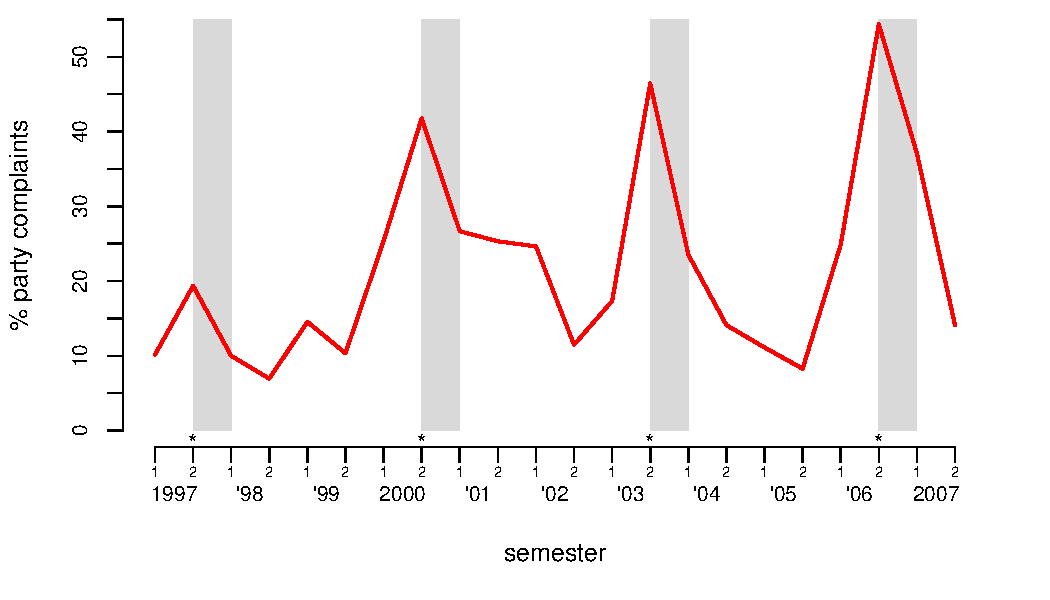
\includegraphics[width=11cm]{c:/data/graphs/ptyComplaints.pdf}
 \caption{\emph{Variation in agenda control.} Party complaints filed at Council General as percentage of
 all issues voted. Grey bars cover electoral semesters and immediate next.}\label{F:ptyComplaints}
 \end{center}
\end{figure}

Movements may also be associated with agenda control. Unlike modern
legislatures or the Supreme Court, IFE has poor control of its
agenda. In particular, parties have standing to file complaints at
IFE which cannot be ignored, diluting members' gatekeeping power.
But there are temporal variations in how well members control their
agenda because the percentage of party complaints filed for the
Council General follows the electoral cycle, as shown in Figure
\ref{F:ptyComplaints}. Defining electoral semesters as those when a
federal election took place and the next (because many complaints
are filed in the immediate aftermath and take some time to be
decided), party complaints as a percentage of all matters voted at
IFE are nearly two-and-a-half times higher in election semesters
than in non-election semesters.\footnote{We relied on Omar
Alejandre's data to produce this differential. We plan to add this
information to our dataset in the immediate future in order to carry
finer-grained analysis.} The percentage fluctuates between 20 and
50\% in the former, between 10 and 20\% in the latter, a
differential we exploit in search of agenda-control effects in
voting patterns. Consistent with our previous discussion, we
speculate that the interaction between principals and agents is
different in electoral than in non-electoral periods. Principals
(ie., parties) not only register more complaints in IFE during
electoral periods, but we also expect that these complaints will
more likely reveal operational preferences and cleavages segmenting
IFE's Council-general. The intuition behind this conjecture is
easier to explain by considering non-electoral semesters.  If better
gatekeeping reduces conflict, as discussed above, then most
decisions that the council-general makes during non-electoral
periods concern routine administrative matters that do not
necessarily map into the north-south dimension that divides party
sponsors and, consequently, IFE councilors.  In contrast, we believe
that electoral times should bring a flurry of activity that increase
the number of politically-consequential matters considered by the
council-general. To test this, we show the distribution of the
absolute value of discrimination parameters across electoral and
non-electoral semesters.  If our conjecture about the importance of
increased agent restraint during non-electoral periods holds any
water, we should see larger average values of discrimination
parameters during electoral semesters. Rows d and e of Table
\ref{T:tests} show the mean and standard deviation of the marginal
posterior distribution of absolute discrimination parameters. We
proceeded as before by dividing the pooled series into electoral
semesters (those where elections are scheduled plus the next one,
$n=7$) and not ($n=13$). We dropped the first semester of each
Council, since these are heavily influenced by our informative
priors on ideal points (but report differentials for the full sample
in rows f and g). As can be seen from the table, discrimination
parameters corresponding to cases in electoral semesters tend to be
larger that those cases that are discussed and decided during
non-electoral semesters.  In fact, a comparison of how often the .95
credible interval for discriminator parameters $\delta$ does not
include the zero value if the case was heard in an electoral or
non-electoral semester (rows i and j of Table \ref{T:tests},
respectively), provides more evidence that cases heard when it is
more difficult to control the agenda are more politically
consequential.

A second implication of agenda control concerns the distribution of
revealed ideal points across electoral and non-electoral semesters.
Because parties should bring more pressure to bear on their
sponsored councilors during electoral periods, we expect
same-sponsor contingents to be more cohesive (ie., their revealed
ideal points to be closer) during electoral than non-electoral
semesters.  Because party divides should be more notable during
electoral periods, we also expect between-party polarization to
increase during electoral semesters.  Finally, we believe that party
pressure over councilors during electoral semesters should lead to a
drop in abstentions during electoral periods, as principals expect
from  their sponsored councilors a fuller commitment to the defense
of their interests.  We estimate within-contingent cohesion by
looking at the posterior marginal distribution of the distance
between the most leftist and most rightist councilors in each
partisan contingent.\footnote{For the sake of simplicity, we refer
to PRI/Green-sponsored councilors as the PRI contingent. The Greens
have been in electoral and legislative alliance with the PRI since
2001, and it is reasonable to view their lone IFE member as a case
of co-sponsorship.} We estimate between-party polarization by
looking at the posterior marginal distribution of the distance
between the centroids of all pairs of partisan contingents, where
the centroids are alternatively defined as the median or average
ideological position of the contingents. Abstention rates are the
share of within-contingent abstentions in a given semester.

\begin{table}
 \begin{center}
  \begin{tabular}{llrrrr}
                  &  & \multicolumn{2}{c}{Electoral} &  \multicolumn{2}{c}{Non-electoral} \\
                  &  & \multicolumn{2}{c}{semester}  &  \multicolumn{2}{c}{semester}      \\
                  &  & Mean      & Std.\ dev.        & Mean    & Std.\ dev.              \\ \hline
   \multicolumn{6}{c}{Within-contingent cohesion}  \\
   PRI    &          &  0.462    & 0.422   &   0.324  &  0.287  \\
   PAN    &          &  0.650    & 0.310   &   0.679  &  0.330  \\
   PRD    &          &  0.979    & 0.183   &   1.120  &  0.230  \\ \hline
   \multicolumn{6}{c}{Between-contingent polarization periods I and II}  \\
   PRI-PAN & medians  &  0.155    & 0.130   &   0.091  &  0.125  \\
           & means   &  0.140    & 0.128   &   0.085  &  0.129  \\
   PRI-PRD &medians  &  0.417    & 0.139   &   0.413  &  0.152  \\
           & means   &  0.441    & 0.141   &   0.434  &  0.161  \\
   PAN-PRD &medians  &  0.262    & 0.163   &   0.323  &  0.170  \\
           & means   &  0.301    & 0.173   &   0.348  &  0.168  \\ \hline
   \multicolumn{6}{c}{Between-contingent polarization period III}  \\
   PRI-PAN & medians &  0.639    & 0.140   &   0.369  &  0.160  \\
           & means   &  0.420    & 0.106   &   0.290  &  0.090  \\ \hline
  \end{tabular}
  \caption{\emph{Partisan contingents within and between.} Posterior marginal mean (standard deviation) of
  within-contingent cohesion and between-contingent polarization. See text.}\label{t:WiAndBtw}
 \end{center}
\end{table}

Table \ref{t:WiAndBtw} displays within-contingent cohesion and
between-contingent polarization statistics.  As we did before, we
drop the first semesters of each council before estimating the
posterior marginal distribution of these statistics.  A glance at
the table shows that evidence supporting the hypothesis that
within-party cohesion increases during electoral semesters is scant.
For PAN- and PRD-sponsored  contingents, within-party cohesion is
barely higher (ie., we observe smaller posterior means) during
electoral semesters, an effect that is not substantively important.
In contrast, PRI-sponsored contingents actually become less cohesive
during electoral semesters.  In fact, we estimate the probability
that cohesion within PRI-sponsored contingents decreases during
electoral semesters to approach 0.61.  In short, we cannot
substantiate the hypothesis that partisan contingents are more
cohesive during electoral semesters.

In contrast, we find some evidence of increased between-contingent
polarization during electoral semesters.  To discuss these results,
we actually distinguish between the two Councils-General, since lack
of a PRD contingent during the second council means that the PRI-PAN
dynamics of polarization are likely to be different across councils.
Be this as it may, we do find that between-party polarization
increases especially for the PRI-PAN dyad in both councils.  When we
consider the distance between the median within the PAN contingent
and the median within the PRI contingent as the relevant indicator
of polarization, we find that this distance increases about 70\% in
both councils. In short, the chances that the PRI-contingent will
vote with the PAN-contingent during electoral semesters are much
reduced in comparison with non-electoral semesters.

Finally, rows k to p of Table \ref{T:tests} present the breakdown of
within-contingent abstention rates across electoral and
non-electoral semesters. Consistent with our hypothesis that
political parties will increase pressure on their contingents to
actively defend their interests, we find that all contingents
decrease their abstention rates during electoral semesters.  This
effect is relatively small for the PAN contingent, a difference of
about 15\% less abstentions during electoral semesters. In contrast,
the contingents of PRI and PRD reduce quite drastically their
abstention rates by about one-third and one-half, respectively,
during electoral semesters. Admittedly, the job of IFE councilors is
to organize elections, and therefore it is no surprise that their
attendance records increase during electoral periods. However, if
these statistics exclusively reflected a problem of job attendance,
we would not expect to see significant cross-party differences.  To
further substantiate our interpretation, we notice that the overall
abstention records of the different partisan contingents are
consistent with our prior notions that the PRI is best at keeping
its contingent in line, followed by the PAN, and the PRD.  Thus, the
abstention records of IFE councilors take on added significance when
we consider the partisan contingents to which they belong.

%% We will need to join Omar's data and our own to analyze delta
%% (discrimination) parameter for party complaints vs rest; or even to
%% estimate ideal point on party complaints exclusively.

%% Preliminary comitee: financiamiento tema==3. Semster by semestre
%% share of divided votes with tema==3.

To summarize, not all our testable implications receive empirical
validation.  With the exception of freshman effects and
within-contingent cohesion scores, however, we find that evidence is
largely consistent with hypotheses of strategic agent behavior.

%% Added to extant evidence on heavy partisan influences in the
%% allegedly non-partisan IFE \citep{estevez.magar.rosas.2008}, the
%% overall picture that emerges is one of relatively capable partisan
%% vetting of potential councilors along with heavy involvement of
%% political parties in signaling their preferences to their sponsored
%% contingents.

\section{Conclusion}

We have used a model designed to estimate ideal point shifts to
investigate voting patterns in a committee whose members represent
the interests of others. Our study found that members' ideal points
shifted significantly over the course of their tenure. If we assume
that voting is sincere, as is standard in this strand of voting
literature, the finding is appears to contradict received wisdom
about principal-agent relations.

We questioned the sincerity of voting assumption. Strategy is likely
to kick in in many different forms, and all invalidate sincere
voting. Committee members need to adapt to any changes in the wishes
of their constituents in order to avoid sanctions. They can also
anticipate what others will do later and decide to cast
sophisticated votes in the early votes of complex agendas. And to
the extent that they retain some control of their agenda, they
should avoid entering political mine fields by removing thorny
issues from the table. They can also trade votes to secure passage
of pieces they deem valuable. All this strategy will push them away
from simply picking the alternative most proximal to their personal
beliefs. So the voting patterns that can be detected will reveal the
working forces of strategic behavior.

We tested some implication of our discussion on the observed
behavior of committee members. Evidence appears to indicate that
drift in our representative council is associated with strategic
considerations, perhaps not at all with changing personal beliefs of
members. Our findings clearly indicate the need to think harder
about the role of strategy in ideal point estimation, especially on
ways to model and estimate its effects in voting.


\section*{Appendix 1: Code for four semesters}

\begin{scriptsize}
\begin{verbatim}
 for (j in 1:J){                                                 ## loop over councilors
   for (i in 1:I){                                               ## loop over items
     y.hat[j,i] ~ dbern(p[j,i]);                                 ## stochastic vote
     p[j,i] <- phi(y.star[j,i]);                                 ## 0<p<1 deterministic part
     y.star[j,i] ~ dnorm(mu[j,i],1)I(lower.y[j,i],upper.y[j,i]); ## truncated normal sampling
                                                                 ## cf. Jackman 2001
     mu[j,i] <- delta[i]*(x1[j]*d1[i] + x2[j]*d2[i]
                        + x3[j]*d3[i] + x4[j]*d4[i]) - n[i];
               ## utility differential: xt's recover t ideal points for member j        ##
               ## dt's are dummies=1 if item voted in semester t (exogenous definition) ##
                 }
     x1[j] ~ dnorm (x0[j],50);              ## Slack S = 1/50 = .02 for all members ##
     x2[j] ~ dnorm (x1[j],50);
     x3[j] ~ dnorm (x2[j],50);
     x4[j] ~ dnorm (x3[j],50);
               }
 for (i in 1:I){
    m[i] <- n[i] / delta[i];                               ## item i's mid-point      ##
               }
 ## priors: give scale and direction to recovered space, see Est�vez et al. 2008 ##
     x0[1] ~ dnorm(0, 1);    #Woldenberg
     x0[2] ~ dnorm(2, 4);    #Barrag�n
     x0[3] ~ dnorm(0, 1);    #Cant�
     x0[4] ~ dnorm(-2, 4);   #C�rdenas
     x0[5] ~ dnorm(0, 1);    #Lujambio
     x0[6] ~ dnorm(0, 1);    #Merino
     x0[7] ~ dnorm(0, 1);    #Molinar
     x0[8] ~ dnorm(0, 1);    #Peschard
     x0[9] ~ dnorm(0, 1);    #Zebad�a
   for(i in 1:I){
       delta[i] ~ dnorm( 0, 0.1);
                }
   for(i in 1:I){
       n[i] ~ dnorm( 0, 0.25);
                }
\end{verbatim}
\end{scriptsize}

\nocite{jackman.2001}

\section*{Appendix 2: $x_{j,t}$ estimates with .80 credible ranges}

%% \begin{figure}
 \begin{center}
  \begin{tabular}{cc}
    \textbf{Periods I and II} &  \textbf{Period III} \\
    \includegraphics[width=.48\textwidth]{c:/data/graphs/1dimDynWold9703jmayorPrecision.pdf}
    &
    \includegraphics[width=.48\textwidth]{c:/data/graphs/1dimDynUgalde0307jmayorPrecision.pdf}
    \\
  \end{tabular}
%%   \caption{\emph{Councilors' ideal points.} Fringes report 80\% credible
%%   range.}\label{F:1by1wCI}
 \end{center}
%% \end{figure}

\begin{footnotesize}

\bibliographystyle{apsr}
\bibliography{harvard}

\end{footnotesize}

\end{document}
